\chapter{Evaluation}

\section{Introduction}

In this chapter, we take a look at the performance characteristics of the two interpreters we created for FrDataFlow. We will explore different types of reactive programs and how they behave under high loads of data, comparing them on a few metrics. More specifically, we will focus on the following two metrics:

\begin{description}[style=nextline]
  \item [Latency]		The time it takes for a value to propagate through the entire graph of signals
  \item [Throughput]	The amount of values that can propagate through the entire graph within a certain time frame.
\end{description}

These objective measurements can provide us with meaningful insight as to how efficient both interpreters are, and what the effects of parallelization are for our benchmarks.

\newpage
\section{Topologies}

Before we can start running benchmarks, we must first define the types of programs that we are interested in profiling. In \cite{drechsler_optimizing_2014}, three topologies are suggested that sufficiently represent any reactive program for the purposes of evaluating performance.

\subsection{Linear}

This model is the simplest one: we have a graph of signals where each signal only has one parent and one child. When the source signal emits a new value, it simply propagates through the graph in one linear motion and stops at the end. 

\begin{figure}[h]
	\centerline{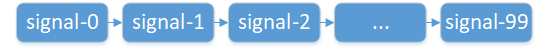
\includegraphics[scale=0.7]{images/Evaluation-Topologies-Linear.png}}
	\caption{A linear topology: each signal has one parent and one child}
	\label{fig:evaluation-topologies-linear}
\end{figure}

\subsection{Fan out}

In this topology, our graph immediately splits up into many children, as shown in figure \ref{fig:evaluation-topologies-fanout}. This is a scenario where one source signal provides important data that every other signal depends upon. The interesting effect of this is when that specific source signal emits a new value, it will trigger an immediate high load of updates for all of its children. 

\begin{figure}[h]
	\centerline{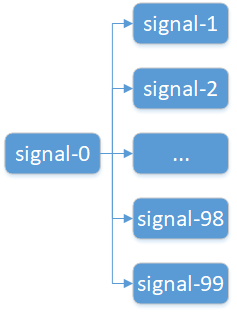
\includegraphics[scale=0.7]{images/Evaluation-Topologies-Fanout.png}}
	\caption{A fan-out topology: one signal with a large amount of children}
	\label{fig:evaluation-topologies-fanout}
\end{figure}


\subsection{Square}

The square topology is expected to be the most common, it provides a signal graph that is not extremely deep such as the linear topology nor is it very wide like the fan-out variant. In this topology, signals have a variable amount of parents and children, shaping the graph into a square. For the purposes of our benchmarks, we will use an exact square graph for simplicity.  

\begin{figure}[h]
	\centerline{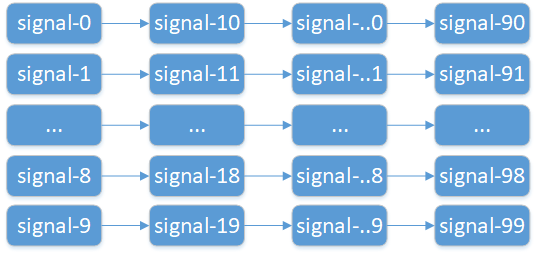
\includegraphics[scale=0.7]{images/Evaluation-Topologies-Square.png}}
	\caption{A square topology: The signal graph is equally deep as it is wide}
	\label{fig:evaluation-topologies-square}
\end{figure}

\section{Without dataflow engine}

\section{With dataflow engine}

\subsection{Without parallelization}

\subsection{With parallelization}

\section{Conclusion}
